% Options for packages loaded elsewhere
% Options for packages loaded elsewhere
\PassOptionsToPackage{unicode}{hyperref}
\PassOptionsToPackage{hyphens}{url}
\PassOptionsToPackage{dvipsnames,svgnames,x11names}{xcolor}
%
\documentclass[
  11pt,
]{article}
\usepackage{xcolor}
\usepackage[margin=1in]{geometry}
\usepackage{amsmath,amssymb}
\setcounter{secnumdepth}{5}
\usepackage{iftex}
\ifPDFTeX
  \usepackage[T1]{fontenc}
  \usepackage[utf8]{inputenc}
  \usepackage{textcomp} % provide euro and other symbols
\else % if luatex or xetex
  \usepackage{unicode-math} % this also loads fontspec
  \defaultfontfeatures{Scale=MatchLowercase}
  \defaultfontfeatures[\rmfamily]{Ligatures=TeX,Scale=1}
\fi
\usepackage{lmodern}
\ifPDFTeX\else
  % xetex/luatex font selection
\fi
% Use upquote if available, for straight quotes in verbatim environments
\IfFileExists{upquote.sty}{\usepackage{upquote}}{}
\IfFileExists{microtype.sty}{% use microtype if available
  \usepackage[]{microtype}
  \UseMicrotypeSet[protrusion]{basicmath} % disable protrusion for tt fonts
}{}
\makeatletter
\@ifundefined{KOMAClassName}{% if non-KOMA class
  \IfFileExists{parskip.sty}{%
    \usepackage{parskip}
  }{% else
    \setlength{\parindent}{0pt}
    \setlength{\parskip}{6pt plus 2pt minus 1pt}}
}{% if KOMA class
  \KOMAoptions{parskip=half}}
\makeatother
% Make \paragraph and \subparagraph free-standing
\makeatletter
\ifx\paragraph\undefined\else
  \let\oldparagraph\paragraph
  \renewcommand{\paragraph}{
    \@ifstar
      \xxxParagraphStar
      \xxxParagraphNoStar
  }
  \newcommand{\xxxParagraphStar}[1]{\oldparagraph*{#1}\mbox{}}
  \newcommand{\xxxParagraphNoStar}[1]{\oldparagraph{#1}\mbox{}}
\fi
\ifx\subparagraph\undefined\else
  \let\oldsubparagraph\subparagraph
  \renewcommand{\subparagraph}{
    \@ifstar
      \xxxSubParagraphStar
      \xxxSubParagraphNoStar
  }
  \newcommand{\xxxSubParagraphStar}[1]{\oldsubparagraph*{#1}\mbox{}}
  \newcommand{\xxxSubParagraphNoStar}[1]{\oldsubparagraph{#1}\mbox{}}
\fi
\makeatother


\usepackage{longtable,booktabs,array}
\usepackage{calc} % for calculating minipage widths
% Correct order of tables after \paragraph or \subparagraph
\usepackage{etoolbox}
\makeatletter
\patchcmd\longtable{\par}{\if@noskipsec\mbox{}\fi\par}{}{}
\makeatother
% Allow footnotes in longtable head/foot
\IfFileExists{footnotehyper.sty}{\usepackage{footnotehyper}}{\usepackage{footnote}}
\makesavenoteenv{longtable}
\usepackage{graphicx}
\makeatletter
\newsavebox\pandoc@box
\newcommand*\pandocbounded[1]{% scales image to fit in text height/width
  \sbox\pandoc@box{#1}%
  \Gscale@div\@tempa{\textheight}{\dimexpr\ht\pandoc@box+\dp\pandoc@box\relax}%
  \Gscale@div\@tempb{\linewidth}{\wd\pandoc@box}%
  \ifdim\@tempb\p@<\@tempa\p@\let\@tempa\@tempb\fi% select the smaller of both
  \ifdim\@tempa\p@<\p@\scalebox{\@tempa}{\usebox\pandoc@box}%
  \else\usebox{\pandoc@box}%
  \fi%
}
% Set default figure placement to htbp
\def\fps@figure{htbp}
\makeatother





\setlength{\emergencystretch}{3em} % prevent overfull lines

\providecommand{\tightlist}{%
  \setlength{\itemsep}{0pt}\setlength{\parskip}{0pt}}



 


\usepackage{booktabs}
\usepackage{longtable}
\usepackage{array}
\usepackage{multirow}
\usepackage{wrapfig}
\usepackage{float}
\usepackage{colortbl}
\usepackage{pdflscape}
\usepackage{tabu}
\usepackage{threeparttable}
\usepackage{threeparttablex}
\usepackage[normalem]{ulem}
\usepackage{makecell}
\usepackage{xcolor}
\usepackage{booktabs}
\usepackage{longtable}
\usepackage{adjustbox}
\usepackage{pdflscape}
\makeatletter
\@ifpackageloaded{caption}{}{\usepackage{caption}}
\AtBeginDocument{%
\ifdefined\contentsname
  \renewcommand*\contentsname{Table of contents}
\else
  \newcommand\contentsname{Table of contents}
\fi
\ifdefined\listfigurename
  \renewcommand*\listfigurename{List of Figures}
\else
  \newcommand\listfigurename{List of Figures}
\fi
\ifdefined\listtablename
  \renewcommand*\listtablename{List of Tables}
\else
  \newcommand\listtablename{List of Tables}
\fi
\ifdefined\figurename
  \renewcommand*\figurename{Figure}
\else
  \newcommand\figurename{Figure}
\fi
\ifdefined\tablename
  \renewcommand*\tablename{Table}
\else
  \newcommand\tablename{Table}
\fi
}
\@ifpackageloaded{float}{}{\usepackage{float}}
\floatstyle{ruled}
\@ifundefined{c@chapter}{\newfloat{codelisting}{h}{lop}}{\newfloat{codelisting}{h}{lop}[chapter]}
\floatname{codelisting}{Listing}
\newcommand*\listoflistings{\listof{codelisting}{List of Listings}}
\makeatother
\makeatletter
\makeatother
\makeatletter
\@ifpackageloaded{caption}{}{\usepackage{caption}}
\@ifpackageloaded{subcaption}{}{\usepackage{subcaption}}
\makeatother
\usepackage{bookmark}
\IfFileExists{xurl.sty}{\usepackage{xurl}}{} % add URL line breaks if available
\urlstyle{same}
\hypersetup{
  pdftitle={Ownership Transfers and Eviction Filing Rates},
  pdfauthor={Philly Evictions Project},
  colorlinks=true,
  linkcolor={blue},
  filecolor={Maroon},
  citecolor={Blue},
  urlcolor={Blue},
  pdfcreator={LaTeX via pandoc}}


\title{Ownership Transfers and Eviction Filing Rates}
\author{Philly Evictions Project}
\date{2026-03-28}
\begin{document}
\maketitle

\renewcommand*\contentsname{Table of contents}
{
\hypersetup{linkcolor=}
\setcounter{tocdepth}{3}
\tableofcontents
}

\section{Overview}\label{overview}

This note reports the streamlined annual transfer-evictions
specification. The main outcome is
\texttt{filing\_rate\ =\ num\_filings\ /\ total\_units} in a full
building-year panel from 2006 to 2019, with single-transfer treated
buildings compared against buildings never transferred in the RTT data.
The omitted event time is \texttt{t\ =\ r\ event\_ref\_period}.

The annual surface has been pruned to four blocks:

\begin{itemize}
\tightlist
\item
  filing-rate event studies
\item
  occupancy, resident-composition, complaint, and permit outcomes
\item
  rent outcomes using the unified and safe series
\item
  rental-evidence event studies for \texttt{1-unit} and
  \texttt{2+\ unit} buildings
\end{itemize}

Portfolio filing types are computed using the helper logic from the
production script, with portfolio size and filing rates defined using
all holdings, including \texttt{1-unit} buildings. The filing and
neighborhood-outcome regressions then restrict the estimation sample as
needed.

\section{Main Filing Results}\label{main-filing-results}

The filing sample grid now separates \texttt{1-unit} properties from the
multifamily stock. The main justification for the \texttt{2+\ unit}
analysis sample is that the \texttt{2+} and \texttt{5+} estimates are
close, while \texttt{1-unit} properties are shown separately as the
single-family contrast and the \texttt{10+} cut is treated as a stricter
appendix validation rather than the main specification.

At \texttt{t\ =\ +1}, the filing-rate coefficient is 0.0089 for
\texttt{2+\ units}, 0.0117 for \texttt{5+\ units}, and 0.0125 for
\texttt{10+\ units}.

\begin{longtable}[t]{lrrr}
\caption{\label{tab:filing-sample-table}Sample sizes for the streamlined annual filing-rate event studies}\\
\toprule
Sample & Rows & Treated PIDs & Control PIDs\\
\midrule
All buildings & 2,598,476 & 66,424 & 123,376\\
1-unit & 1,956,298 & 51,378 & 90,413\\
2+ units & 642,173 & 15,051 & 32,976\\
2+ units, rental evidence & 340,761 & 13,319 & 28,792\\
5+ units & 82,762 & 1,543 & 5,089\\
\addlinespace
5+ units, rental evidence & 37,797 & 1,216 & 3,874\\
10+ units & 38,376 & 713 & 2,551\\
10+ units, rental evidence & 18,570 & 548 & 1,923\\
\bottomrule
\end{longtable}

\begin{figure}[H]

{\centering 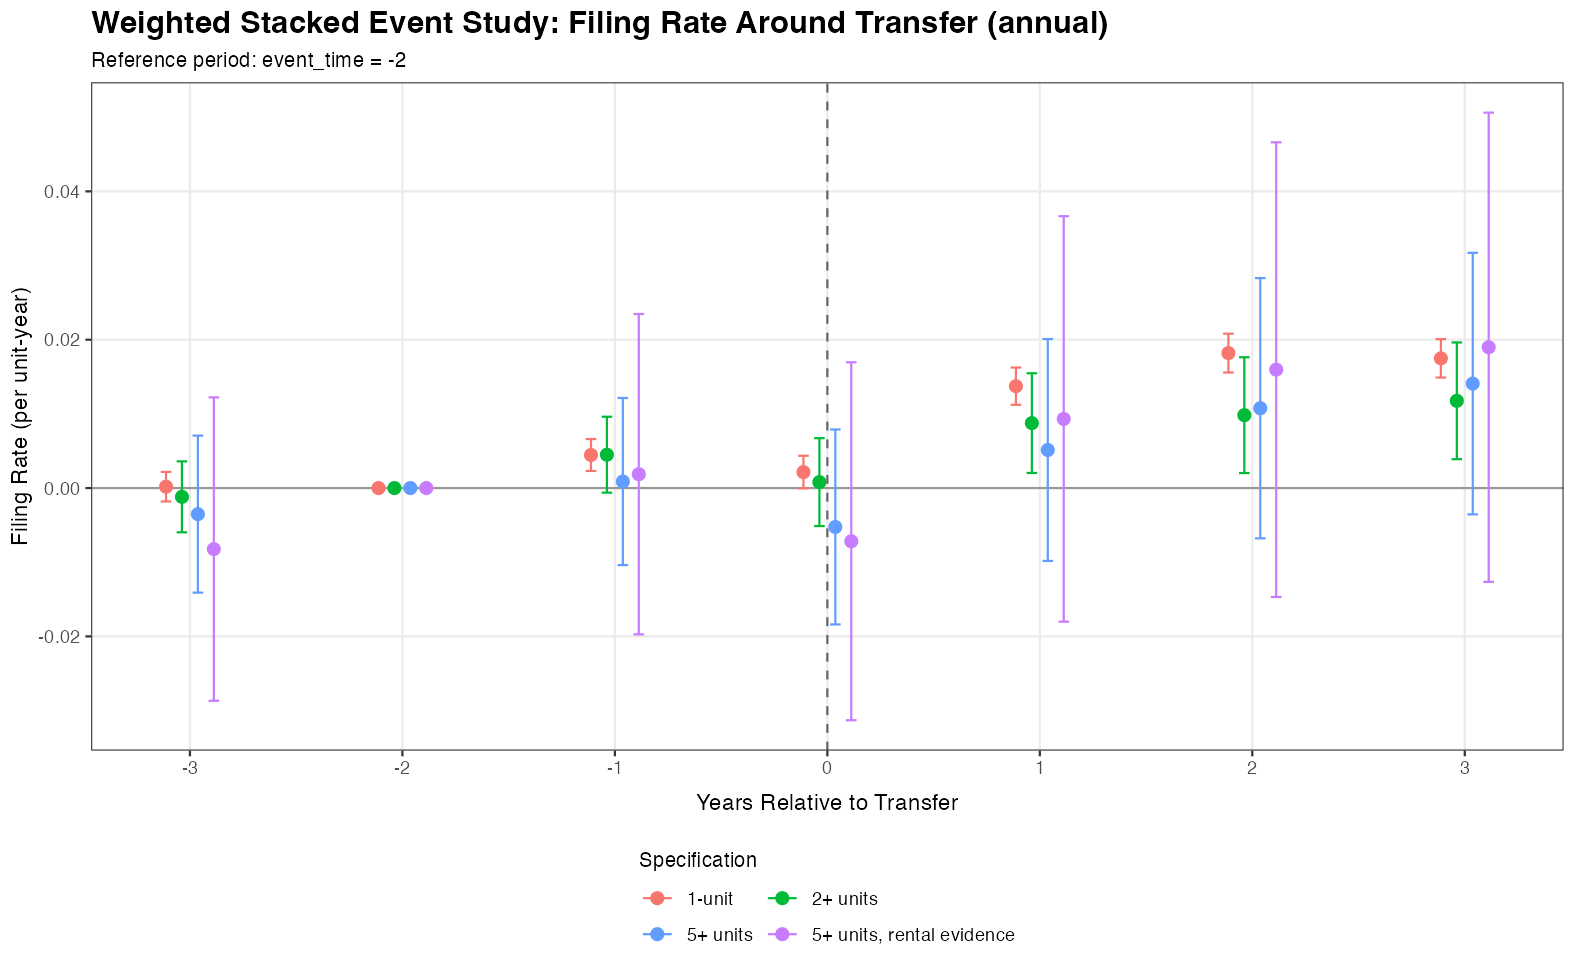
\includegraphics[width=0.95\linewidth,height=\textheight,keepaspectratio]{../output/transfer_evictions/figs/rtt_annual_filing_core.png}

}

\caption{Annual filing-rate event study by sample restriction. The main
comparison is 2+ units versus 5+ units; 10+ is included as a stricter
appendix check.}

\end{figure}%

\scriptsize
\begin{adjustbox}{max width=\textwidth}

\begingroup
\centering
\begin{tabular}{lcccccccc}
   \toprule
    & \multicolumn{8}{c}{filing\_rate}\\
   Sample             & All buildings   & 1-unit          & 2+ units       & 2+ units, rental evidence & 5+ units       & 5+ units, rental evidence & 10+ units     & 10+ units, rental evidence \\   
                      & (1)             & (2)             & (3)            & (4)                       & (5)            & (6)                       & (7)           & (8)\\  
   \midrule 
   et\_m3             & -0.0032$^{***}$ & -0.0045$^{***}$ & -0.0019        & 0.0019                    & -0.0037        & -0.0057                   & -0.0030       & -0.0045\\   
                      & (0.0010)        & (0.0010)        & (0.0017)       & (0.0039)                  & (0.0035)       & (0.0076)                  & (0.0043)      & (0.0089)\\   
   et\_m1             & 0.0023$^{**}$   & 0.0051$^{***}$  & -0.0003        & 0.0093$^{*}$              & -0.0033        & -0.0030                   & -0.0024       & -0.0023\\   
                      & (0.0012)        & (0.0010)        & (0.0021)       & (0.0050)                  & (0.0044)       & (0.0092)                  & (0.0053)      & (0.0107)\\   
   et\_0              & -0.0009         & -0.0015         & -0.0002        & 0.0042                    & -0.0013        & 0.0006                    & -0.0015       & 0.0002\\   
                      & (0.0010)        & (0.0010)        & (0.0018)       & (0.0039)                  & (0.0037)       & (0.0074)                  & (0.0045)      & (0.0086)\\   
   et\_1              & 0.0120$^{***}$  & 0.0151$^{***}$  & 0.0089$^{***}$ & 0.0165$^{***}$            & 0.0117$^{**}$  & 0.0212$^{**}$             & 0.0125$^{**}$ & 0.0228$^{**}$\\   
                      & (0.0014)        & (0.0012)        & (0.0024)       & (0.0049)                  & (0.0050)       & (0.0093)                  & (0.0061)      & (0.0108)\\   
   et\_2              & 0.0143$^{***}$  & 0.0216$^{***}$  & 0.0073$^{***}$ & 0.0103$^{**}$             & 0.0103$^{*}$   & 0.0160                    & 0.0080        & 0.0128\\   
                      & (0.0015)        & (0.0013)        & (0.0027)       & (0.0051)                  & (0.0057)       & (0.0098)                  & (0.0066)      & (0.0112)\\   
   et\_3              & 0.0146$^{***}$  & 0.0187$^{***}$  & 0.0107$^{***}$ & 0.0145$^{***}$            & 0.0145$^{**}$  & 0.0214$^{**}$             & 0.0126$^{*}$  & 0.0191$^{*}$\\   
                      & (0.0016)        & (0.0014)        & (0.0028)       & (0.0051)                  & (0.0059)       & (0.0098)                  & (0.0068)      & (0.0113)\\   
   et\_4              & 0.0146$^{***}$  & 0.0203$^{***}$  & 0.0091$^{***}$ & 0.0110$^{***}$            & 0.0095$^{*}$   & 0.0128$^{*}$              & 0.0073        & 0.0108\\   
                      & (0.0015)        & (0.0015)        & (0.0025)       & (0.0040)                  & (0.0049)       & (0.0076)                  & (0.0056)      & (0.0087)\\   
   et\_5              & 0.0126$^{***}$  & 0.0134$^{***}$  & 0.0117$^{***}$ & 0.0137$^{***}$            & 0.0143$^{***}$ & 0.0192$^{**}$             & 0.0139$^{**}$ & 0.0190$^{**}$\\   
                      & (0.0015)        & (0.0015)        & (0.0026)       & (0.0041)                  & (0.0055)       & (0.0081)                  & (0.0064)      & (0.0095)\\   
    \\
   Observations       & 2,598,476       & 1,956,298       & 642,173        & 340,761                   & 82,762         & 37,797                    & 38,376        & 18,570\\  
   R$^2$              & 0.33369         & 0.22100         & 0.52039        & 0.54546                   & 0.69746        & 0.69015                   & 0.70744       & 0.69125\\  
   Within R$^2$       & 0.00039         & 0.00048         & 0.00036        & 0.00039                   & 0.00085        & 0.00114                   & 0.00086       & 0.00127\\  
    \\
   PID fixed effects  & $\checkmark$    & $\checkmark$    & $\checkmark$   & $\checkmark$              & $\checkmark$   & $\checkmark$              & $\checkmark$  & $\checkmark$\\   
   year fixed effects & $\checkmark$    & $\checkmark$    & $\checkmark$   & $\checkmark$              & $\checkmark$   & $\checkmark$              & $\checkmark$  & $\checkmark$\\   
   \bottomrule
\end{tabular}
\par\endgroup



\end{adjustbox}

\begin{longtable}[t]{lrrr}
\caption{\label{tab:filing-core-summary}Selected filing-rate coefficients from the streamlined sample grid}\\
\toprule
Sample & t+1 & t+2 & t+3\\
\midrule
1-unit & 0.0151 & 0.0216 & 0.0187\\
10+ units & 0.0125 & 0.0080 & 0.0126\\
10+ units, rental evidence & 0.0228 & 0.0128 & 0.0190\\
2+ units & 0.0089 & 0.0073 & 0.0107\\
2+ units, rental evidence & 0.0165 & 0.0103 & 0.0145\\
\addlinespace
5+ units & 0.0117 & 0.0103 & 0.0145\\
5+ units, rental evidence & 0.0212 & 0.0160 & 0.0214\\
\bottomrule
\end{longtable}

\section{Filing Heterogeneity by Acquirer
Type}\label{filing-heterogeneity-by-acquirer-type}

The main heterogeneity split uses four acquirer types:

\begin{itemize}
\tightlist
\item
  \texttt{High-filer\ portfolio}
\item
  \texttt{Low-filer\ portfolio}
\item
  \texttt{Small\ portfolio}
\item
  \texttt{Single-purchase}
\end{itemize}

These categories are defined from the helper-function leave-one-out
portfolio measures, while the regression itself is restricted to
\texttt{2+\ unit} buildings. In the current annual outputs, the
\texttt{t\ =\ +2} coefficient is 0.0237 for high-filer portfolios and
-0.0062 for low-filer portfolios.

\begin{figure}[H]

{\centering 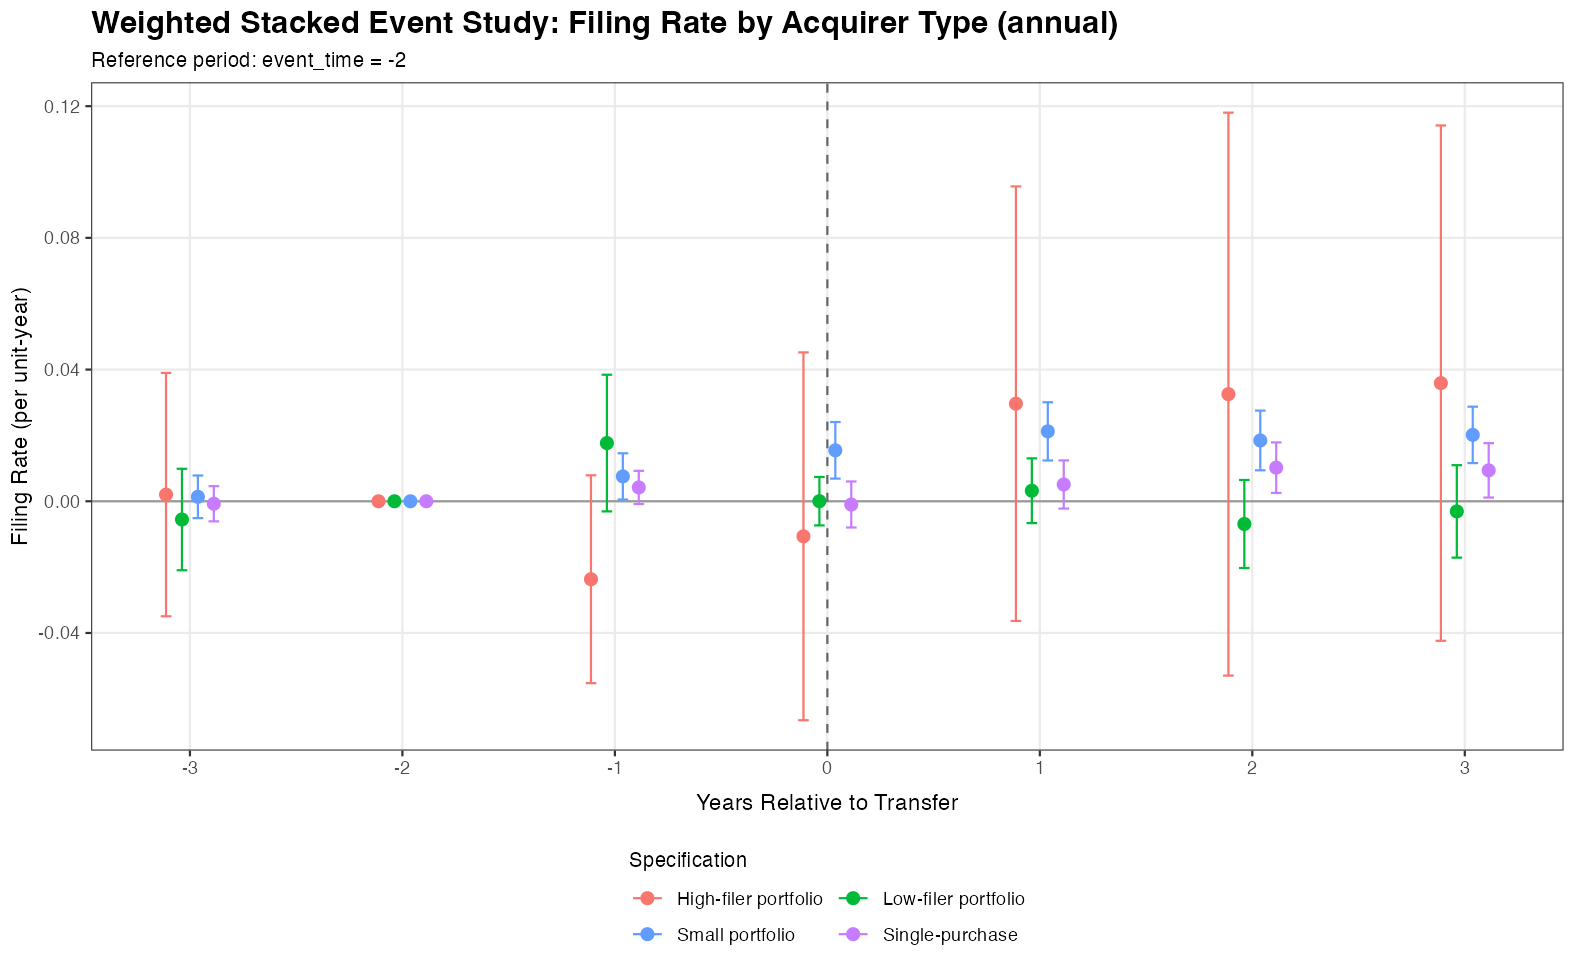
\includegraphics[width=0.95\linewidth,height=\textheight,keepaspectratio]{../output/transfer_evictions/figs/rtt_annual_filing_acq_2plus.png}

}

\caption{Annual filing-rate event study for 2+ unit buildings, split by
acquirer filing type. Controls are never-transferred buildings in the
same 2+ unit sample.}

\end{figure}%

\scriptsize
\begin{adjustbox}{max width=\textwidth}

\begingroup
\centering
\begin{tabular}{lccccc}
   \toprule
    & \multicolumn{5}{c}{filing\_rate}\\
   Acquirer type      & All acquirers  & High-filer portfolio & Low-filer portfolio   & Small portfolio & Single-purchase \\   
                      & (1)            & (2)                  & (3)                   & (4)             & (5)\\  
   \midrule 
   et\_m3             & -0.0018        & -0.0067              & -0.0036               & -0.0044         & 0.0001\\   
                      & (0.0017)       & (0.0130)             & (0.0033)              & (0.0038)        & (0.0018)\\   
   et\_m1             & -0.0002        & -0.0274$^{*}$        & 0.0155$^{*}$          & -0.0030         & 0.0017\\   
                      & (0.0021)       & (0.0144)             & (0.0086)              & (0.0035)        & (0.0018)\\   
   et\_0              & -0.0002        & -0.0109              & 0.0003                & 0.0010          & 0.0011\\   
                      & (0.0018)       & (0.0137)             & (0.0026)              & (0.0032)        & (0.0018)\\   
   et\_1              & 0.0089$^{***}$ & 0.0416$^{**}$        & 0.0025                & 0.0070$^{**}$   & 0.0062$^{***}$\\   
                      & (0.0024)       & (0.0185)             & (0.0056)              & (0.0035)        & (0.0024)\\   
   et\_2              & 0.0076$^{***}$ & 0.0237               & -0.0062$^{*}$         & 0.0071$^{*}$    & 0.0085$^{***}$\\   
                      & (0.0027)       & (0.0206)             & (0.0034)              & (0.0041)        & (0.0031)\\   
   et\_3              & 0.0101$^{***}$ & 0.0289$^{**}$        & -0.0046               & 0.0134$^{**}$   & 0.0099$^{***}$\\   
                      & (0.0028)       & (0.0145)             & (0.0041)              & (0.0055)        & (0.0036)\\   
   et\_4              & 0.0092$^{***}$ & 0.0013               & 0.0061                & 0.0181$^{**}$   & 0.0090$^{***}$\\   
                      & (0.0025)       & (0.0151)             & (0.0045)              & (0.0073)        & (0.0027)\\   
   et\_5              & 0.0112$^{***}$ & 0.0305$^{*}$         & -0.0030               & 0.0228$^{***}$  & 0.0089$^{***}$\\   
                      & (0.0027)       & (0.0164)             & (0.0029)              & (0.0077)        & (0.0029)\\   
    \\
   Observations       & 640,544        & 451,695              & 459,341               & 482,530         & 570,594\\  
   R$^2$              & 0.52045        & 0.54675              & 0.53557               & 0.52768         & 0.52079\\  
   Within R$^2$       & 0.00034        & 0.00063              & $7.83\times 10^{-5}$  & 0.00016         & 0.00019\\  
    \\
   PID fixed effects  & $\checkmark$   & $\checkmark$         & $\checkmark$          & $\checkmark$    & $\checkmark$\\   
   year fixed effects & $\checkmark$   & $\checkmark$         & $\checkmark$          & $\checkmark$    & $\checkmark$\\   
   \bottomrule
\end{tabular}
\par\endgroup



\end{adjustbox}

\begin{longtable}[t]{lrrr}
\caption{\label{tab:filing-acq-summary}Selected 2+ unit filing-rate coefficients by acquirer type}\\
\toprule
Acquirer type & t+1 & t+2 & t+3\\
\midrule
All acquirers & 0.0089 & 0.0076 & 0.0101\\
High-filer portfolio & 0.0416 & 0.0237 & 0.0289\\
Low-filer portfolio & 0.0025 & -0.0062 & -0.0046\\
Single-purchase & 0.0062 & 0.0085 & 0.0099\\
Small portfolio & 0.0070 & 0.0071 & 0.0134\\
\bottomrule
\end{longtable}

\section{Weighted Stacked Robustness}\label{weighted-stacked-robustness}

As a robustness check, the production script now runs a weighted stacked
annual filing-rate estimator for the full sample and the
\texttt{2+\ unit} sample. This is not the main specification, but it
provides a cleaner stacked benchmark than the earlier scratch
implementation.

For the \texttt{2+\ unit} weighted stacked regression, the
\texttt{t\ =\ -3} coefficient is -0.0009 and the \texttt{t\ =\ +2}
coefficient is 0.0124.

\begin{figure}[H]

{\centering \includegraphics[width=0.95\linewidth,height=\textheight,keepaspectratio]{../output/transfer_evictions/figs/rtt_annual_baseline_stacked_weighted.png}

}

\caption{Weighted stacked annual filing-rate event study. Corrective
weights are applied at the cohort-control level; the main comparison is
the full sample versus 2+ units.}

\end{figure}%

\scriptsize
\begin{adjustbox}{max width=\textwidth}

\begingroup
\centering
\begin{tabular}{lcc}
   \toprule
    & \multicolumn{2}{c}{filing\_rate}\\
   Sample                     & All buildings (weighted stacked) & 2+ unit buildings (weighted stacked) \\   
                              & (1)                              & (2)\\  
   \midrule 
   st\_et\_m3                 & -0.0005                          & -0.0009\\   
                              & (0.0015)                         & (0.0026)\\   
   st\_et\_m1                 & 0.0056$^{***}$                   & 0.0052$^{*}$\\   
                              & (0.0016)                         & (0.0027)\\   
   st\_et\_0                  & 0.0017                           & 0.0008\\   
                              & (0.0018)                         & (0.0032)\\   
   st\_et\_1                  & 0.0151$^{***}$                   & 0.0096$^{***}$\\   
                              & (0.0021)                         & (0.0037)\\   
   st\_et\_2                  & 0.0195$^{***}$                   & 0.0124$^{**}$\\   
                              & (0.0027)                         & (0.0049)\\   
   st\_et\_3                  & 0.0199$^{***}$                   & 0.0137$^{***}$\\   
                              & (0.0025)                         & (0.0045)\\   
    \\
   Observations               & 6,960,484                        & 1,811,495\\  
   R$^2$                      & 0.44371                          & 0.62041\\  
   Within R$^2$               & $8\times 10^{-5}$                & $6.61\times 10^{-5}$\\   
    \\
   pid\_cohort fixed effects  & $\checkmark$                     & $\checkmark$\\   
   yr\_cohort fixed effects   & $\checkmark$                     & $\checkmark$\\   
   \bottomrule
\end{tabular}
\par\endgroup



\end{adjustbox}

\begingroup\fontsize{8}{10}\selectfont

\begin{longtable}[t]{lrrrr}
\caption{\label{tab:filing-stacked-qweights}Weighted stacked annual filing-rate cohort weights}\\
\toprule
Sample & Cohort & Treated PIDs & Control PIDs & Corrective weight\\
\midrule
All buildings & 2009 & 3105 & 120499 & 0.785\\
All buildings & 2010 & 3133 & 120831 & 0.790\\
All buildings & 2011 & 2942 & 121150 & 0.740\\
All buildings & 2012 & 3502 & 121585 & 0.877\\
All buildings & 2013 & 3997 & 122025 & 0.998\\
\addlinespace
All buildings & 2014 & 4493 & 122470 & 1.117\\
All buildings & 2015 & 4926 & 122902 & 1.221\\
All buildings & 2016 & 5908 & 123264 & 1.460\\
2+ units & 2009 & 685 & 31555 & 0.763\\
2+ units & 2010 & 701 & 31747 & 0.776\\
\addlinespace
2+ units & 2011 & 711 & 31910 & 0.783\\
2+ units & 2012 & 875 & 32092 & 0.958\\
2+ units & 2013 & 950 & 32266 & 1.035\\
2+ units & 2014 & 1038 & 32452 & 1.124\\
2+ units & 2015 & 1108 & 32667 & 1.192\\
\addlinespace
2+ units & 2016 & 1262 & 32875 & 1.349\\
\bottomrule
\end{longtable}
\endgroup{}

\section{Occupancy, Demographics, Complaints, and
Permits}\label{occupancy-demographics-complaints-and-permits}

These outcomes are estimated on the \texttt{2+\ unit} sample and split
by the same acquirer-type bins as the filing regressions. The output
surface here is intentionally narrower than the earlier report: the
focus is occupancy, resident composition, complaints, and permits.

\begin{figure}[H]

{\centering \includegraphics[width=0.95\linewidth,height=\textheight,keepaspectratio]{../output/transfer_evictions/figs/rtt_annual_occupancy_2plus.png}

}

\caption{Occupancy-rate event study for 2+ unit buildings, overall and
by acquirer filing type.}

\end{figure}%

\scriptsize
\begin{adjustbox}{max width=\textwidth}

\begingroup
\centering
\begin{tabular}{lccccc}
   \toprule
    & \multicolumn{5}{c}{occupancy\_rate}\\
   Acquirer type      & All acquirers   & High-filer portfolio & Low-filer portfolio & Small portfolio & Single-purchase \\   
                      & (1)             & (2)                  & (3)                 & (4)             & (5)\\  
   \midrule 
   et\_m3             & 0.0031          & -0.0221              & -0.0052             & -0.0181$^{***}$ & 0.0102\\   
                      & (0.0067)        & (0.0265)             & (0.0175)            & (0.0067)        & (0.0092)\\   
   et\_m1             & -0.0053         & -0.0458              & -0.0413$^{*}$       & -0.0169$^{**}$  & 0.0077\\   
                      & (0.0071)        & (0.0301)             & (0.0214)            & (0.0082)        & (0.0092)\\   
   et\_0              & -0.0155$^{**}$  & -0.0280              & -0.0824$^{***}$     & -0.0215$^{**}$  & -0.0021\\   
                      & (0.0075)        & (0.0312)             & (0.0237)            & (0.0087)        & (0.0096)\\   
   et\_1              & -0.0270$^{***}$ & -0.0405              & -0.1041$^{***}$     & -0.0214$^{**}$  & -0.0139\\   
                      & (0.0084)        & (0.0328)             & (0.0270)            & (0.0092)        & (0.0108)\\   
   et\_2              & -0.0314$^{***}$ & -0.0722$^{**}$       & -0.1086$^{***}$     & -0.0271$^{***}$ & -0.0145\\   
                      & (0.0086)        & (0.0349)             & (0.0278)            & (0.0087)        & (0.0109)\\   
   et\_3              & -0.0392$^{***}$ & -0.0963$^{**}$       & -0.1025$^{***}$     & -0.0356$^{***}$ & -0.0237$^{**}$\\   
                      & (0.0097)        & (0.0425)             & (0.0314)            & (0.0089)        & (0.0120)\\   
   et\_4              & -0.0324$^{***}$ & -0.0300              & -0.1120$^{***}$     & -0.0526$^{***}$ & -0.0173\\   
                      & (0.0096)        & (0.0284)             & (0.0284)            & (0.0089)        & (0.0127)\\   
   et\_5              & -0.0419$^{***}$ & -0.0091              & -0.0745$^{***}$     & -0.0739$^{***}$ & -0.0401$^{***}$\\   
                      & (0.0070)        & (0.0260)             & (0.0170)            & (0.0100)        & (0.0093)\\   
    \\
   Observations       & 640,544         & 451,695              & 459,341             & 482,530         & 570,594\\  
   R$^2$              & 0.50791         & 0.49361              & 0.50079             & 0.49636         & 0.50579\\  
   Within R$^2$       & 0.00098         & 0.00039              & 0.00148             & 0.00030         & 0.00038\\  
    \\
   PID fixed effects  & $\checkmark$    & $\checkmark$         & $\checkmark$        & $\checkmark$    & $\checkmark$\\   
   year fixed effects & $\checkmark$    & $\checkmark$         & $\checkmark$        & $\checkmark$    & $\checkmark$\\   
   \bottomrule
\end{tabular}
\par\endgroup



\end{adjustbox}

\begin{figure}[H]

{\centering \includegraphics[width=0.95\linewidth,height=\textheight,keepaspectratio]{../output/transfer_evictions/figs/rtt_annual_pct_black_2plus.png}

}

\caption{Share Black residents for 2+ unit buildings, overall and by
acquirer filing type.}

\end{figure}%

\begin{figure}[H]

{\centering \includegraphics[width=0.95\linewidth,height=\textheight,keepaspectratio]{../output/transfer_evictions/figs/rtt_annual_pct_latino_2plus.png}

}

\caption{Share Latino residents for 2+ unit buildings, overall and by
acquirer filing type.}

\end{figure}%

\begin{figure}[H]

{\centering \includegraphics[width=0.95\linewidth,height=\textheight,keepaspectratio]{../output/transfer_evictions/figs/rtt_annual_pct_white_2plus.png}

}

\caption{Share White residents for 2+ unit buildings, overall and by
acquirer filing type.}

\end{figure}%

\begin{figure}[H]

{\centering \includegraphics[width=0.95\linewidth,height=\textheight,keepaspectratio]{../output/transfer_evictions/figs/rtt_annual_pct_asian_2plus.png}

}

\caption{Share Asian residents for 2+ unit buildings, overall and by
acquirer filing type.}

\end{figure}%

\begin{figure}[H]

{\centering \includegraphics[width=0.95\linewidth,height=\textheight,keepaspectratio]{../output/transfer_evictions/figs/rtt_annual_permit_rate_2plus.png}

}

\caption{Permit-rate event study for 2+ unit buildings, overall and by
acquirer filing type.}

\end{figure}%

\begin{figure}[H]

{\centering \includegraphics[width=0.95\linewidth,height=\textheight,keepaspectratio]{../output/transfer_evictions/figs/rtt_annual_complaint_rate_2plus.png}

}

\caption{Complaint-rate event study for 2+ unit buildings, overall and
by acquirer filing type.}

\end{figure}%

\section{Rent Outcomes}\label{rent-outcomes}

The rent analysis is run on all units, but treated buildings are
required to have both pre- and post-acquisition support in the relevant
rent measure. The report keeps both the unified rent series and the safe
single-source series.

\begin{figure}[H]

{\centering \includegraphics[width=0.95\linewidth,height=\textheight,keepaspectratio]{../output/transfer_evictions/figs/rtt_annual_rent_core.png}

}

\caption{Log median rent event study, all units, overall and by acquirer
filing type.}

\end{figure}%

\scriptsize
\begin{adjustbox}{max width=\textwidth}

\begingroup
\centering
\begin{tabular}{lccccc}
   \toprule
    & \multicolumn{5}{c}{log\_med\_rent}\\
   Acquirer type      & All acquirers  & High-filer portfolio & Low-filer portfolio & Small portfolio & Single-purchase \\   
                      & (1)            & (2)                  & (3)                 & (4)             & (5)\\  
   \midrule 
   et\_m3             & -0.0120        & 0.0272               & 0.0484              & -0.0318         & -0.0415$^{***}$\\   
                      & (0.0147)       & (0.0239)             & (0.0691)            & (0.0222)        & (0.0151)\\   
   et\_m1             & -0.0056        & 0.0162               & -0.0251             & -0.0113         & -0.0103\\   
                      & (0.0091)       & (0.0153)             & (0.0483)            & (0.0177)        & (0.0116)\\   
   et\_0              & 0.0025         & 0.0123               & 0.0424$^{***}$      & -0.0270         & -0.0035\\   
                      & (0.0093)       & (0.0145)             & (0.0161)            & (0.0245)        & (0.0142)\\   
   et\_1              & 0.0116         & 0.0152               & 0.0471$^{*}$        & 0.0380$^{***}$  & -0.0045\\   
                      & (0.0101)       & (0.0137)             & (0.0257)            & (0.0127)        & (0.0160)\\   
   et\_2              & 0.0610$^{***}$ & 0.0549$^{***}$       & 0.1991$^{***}$      & 0.0348$^{**}$   & 0.0343$^{**}$\\   
                      & (0.0175)       & (0.0173)             & (0.0648)            & (0.0156)        & (0.0163)\\   
   et\_3              & 0.0499$^{**}$  & 0.0405$^{**}$        & 0.1901$^{***}$      & 0.0183          & 0.0179\\   
                      & (0.0209)       & (0.0176)             & (0.0697)            & (0.0192)        & (0.0190)\\   
   et\_4              & 0.0360$^{***}$ & 0.0425$^{***}$       & 0.0934$^{**}$       & -0.0380         & 0.0330$^{*}$\\   
                      & (0.0132)       & (0.0156)             & (0.0392)            & (0.0423)        & (0.0192)\\   
   et\_5              & 0.0185         & 0.0129               & 0.0874$^{*}$        & -0.0155         & 0.0160\\   
                      & (0.0153)       & (0.0177)             & (0.0530)            & (0.0218)        & (0.0290)\\   
    \\
   Observations       & 130,946        & 117,300              & 116,488             & 118,763         & 122,939\\  
   R$^2$              & 0.88881        & 0.88833              & 0.88650             & 0.88770         & 0.88985\\  
   Within R$^2$       & 0.00273        & 0.00059              & 0.00462             & 0.00039         & 0.00109\\  
    \\
   PID fixed effects  & $\checkmark$   & $\checkmark$         & $\checkmark$        & $\checkmark$    & $\checkmark$\\   
   year fixed effects & $\checkmark$   & $\checkmark$         & $\checkmark$        & $\checkmark$    & $\checkmark$\\   
   \bottomrule
\end{tabular}
\par\endgroup



\end{adjustbox}

\begin{figure}[H]

{\centering \includegraphics[width=0.95\linewidth,height=\textheight,keepaspectratio]{../output/transfer_evictions/figs/rtt_annual_rent_safe_core.png}

}

\caption{Log median rent (safe single-source series) event study, all
units, overall and by acquirer filing type.}

\end{figure}%

\scriptsize
\begin{adjustbox}{max width=\textwidth}

\begingroup
\centering
\begin{tabular}{lccccc}
   \toprule
    & \multicolumn{5}{c}{log\_med\_rent\_safe}\\
   Acquirer type      & All acquirers  & High-filer portfolio & Low-filer portfolio & Small portfolio & Single-purchase \\   
                      & (1)            & (2)                  & (3)                 & (4)             & (5)\\  
   \midrule 
   et\_m3             & -0.0304        & -0.0176              & 0.0760              & -0.0648$^{***}$ & -0.0415$^{**}$\\   
                      & (0.0188)       & (0.0283)             & (0.1121)            & (0.0219)        & (0.0193)\\   
   et\_m1             & -0.0192$^{*}$  & -0.0184              & -0.0419             & -0.0389         & -0.0109\\   
                      & (0.0112)       & (0.0291)             & (0.0331)            & (0.0284)        & (0.0135)\\   
   et\_0              & -0.0289$^{**}$ & -0.0512$^{**}$       & 0.0766              & -0.0966$^{**}$  & -0.0242\\   
                      & (0.0139)       & (0.0222)             & (0.0562)            & (0.0410)        & (0.0173)\\   
   et\_1              & -0.0047        & -0.0243              & 0.1173$^{*}$        & -0.0046         & -0.0146\\   
                      & (0.0151)       & (0.0288)             & (0.0674)            & (0.0244)        & (0.0179)\\   
   et\_2              & 0.0334$^{*}$   & 0.0030               & 0.1340              & -0.0333         & 0.0350$^{*}$\\   
                      & (0.0183)       & (0.0425)             & (0.0970)            & (0.0217)        & (0.0209)\\   
   et\_3              & 0.0305         & -0.0303              & 0.1634              & -0.0013         & 0.0268\\   
                      & (0.0236)       & (0.0327)             & (0.1058)            & (0.0278)        & (0.0226)\\   
   et\_4              & 0.0441$^{**}$  & -0.0198              & 0.1698$^{**}$       & -0.0203         & 0.0619$^{**}$\\   
                      & (0.0215)       & (0.0263)             & (0.0862)            & (0.0221)        & (0.0275)\\   
   et\_5              & 0.0520         & -0.0031              & 0.2769$^{***}$      & -0.0191         & 0.0590\\   
                      & (0.0333)       & (0.0213)             & (0.0832)            & (0.0198)        & (0.0634)\\   
    \\
   Observations       & 92,561         & 85,909               & 85,733              & 86,869          & 89,257\\  
   R$^2$              & 0.91687        & 0.91663              & 0.91580             & 0.91662         & 0.91804\\  
   Within R$^2$       & 0.00274        & 0.00037              & 0.00330             & 0.00076         & 0.00209\\  
    \\
   PID fixed effects  & $\checkmark$   & $\checkmark$         & $\checkmark$        & $\checkmark$    & $\checkmark$\\   
   year fixed effects & $\checkmark$   & $\checkmark$         & $\checkmark$        & $\checkmark$    & $\checkmark$\\   
   \bottomrule
\end{tabular}
\par\endgroup



\end{adjustbox}

\section{Rental Evidence}\label{rental-evidence}

These regressions show the probability of observed rental evidence
separately for \texttt{1-unit} and \texttt{2+\ unit} buildings. This is
the direct check on the concern that transfers mechanically enter
properties into the observed rental market.

\begin{figure}[H]

{\centering \includegraphics[width=0.95\linewidth,height=\textheight,keepaspectratio]{../output/transfer_evictions/figs/rtt_annual_rental_evidence_1unit.png}

}

\caption{Probability of rental evidence for 1-unit buildings, overall
and by acquirer filing type.}

\end{figure}%

\scriptsize
\begin{adjustbox}{max width=\textwidth}

\begingroup
\centering
\begin{tabular}{lccccc}
   \toprule
    & \multicolumn{5}{c}{has\_rental\_evidence}\\
   Acquirer type      & All acquirers   & High-filer portfolio & Low-filer portfolio & Small portfolio & Single-purchase \\   
                      & (1)             & (2)                  & (3)                 & (4)             & (5)\\  
   \midrule 
   et\_m3             & -0.0629$^{***}$ & -0.2054$^{***}$      & -0.1148$^{***}$     & -0.0999$^{***}$ & -0.0327$^{***}$\\   
                      & (0.0018)        & (0.0083)             & (0.0049)            & (0.0034)        & (0.0024)\\   
   et\_m1             & -0.1340$^{***}$ & -0.3139$^{***}$      & -0.1826$^{***}$     & -0.1832$^{***}$ & -0.0896$^{***}$\\   
                      & (0.0022)        & (0.0089)             & (0.0065)            & (0.0041)        & (0.0029)\\   
   et\_0              & 0.0153$^{***}$  & 0.0333$^{**}$        & 0.1419$^{***}$      & 0.0609$^{***}$  & -0.0102$^{***}$\\   
                      & (0.0030)        & (0.0135)             & (0.0106)            & (0.0063)        & (0.0037)\\   
   et\_1              & 0.0928$^{***}$  & 0.2625$^{***}$       & 0.3856$^{***}$      & 0.2246$^{***}$  & 0.0032\\   
                      & (0.0033)        & (0.0121)             & (0.0110)            & (0.0068)        & (0.0041)\\   
   et\_2              & 0.1091$^{***}$  & 0.2667$^{***}$       & 0.4093$^{***}$      & 0.2505$^{***}$  & 0.0179$^{***}$\\   
                      & (0.0031)        & (0.0108)             & (0.0107)            & (0.0066)        & (0.0039)\\   
   et\_3              & 0.1009$^{***}$  & 0.2340$^{***}$       & 0.3765$^{***}$      & 0.2381$^{***}$  & 0.0194$^{***}$\\   
                      & (0.0029)        & (0.0096)             & (0.0107)            & (0.0064)        & (0.0037)\\   
   et\_4              & 0.0872$^{***}$  & 0.1936$^{***}$       & 0.3131$^{***}$      & 0.2062$^{***}$  & 0.0222$^{***}$\\   
                      & (0.0026)        & (0.0084)             & (0.0106)            & (0.0059)        & (0.0033)\\   
   et\_5              & 0.0719$^{***}$  & 0.1643$^{***}$       & 0.2320$^{***}$      & 0.1621$^{***}$  & 0.0248$^{***}$\\   
                      & (0.0022)        & (0.0065)             & (0.0097)            & (0.0051)        & (0.0028)\\   
    \\
   Observations       & 1,259,297       & 830,325              & 834,388             & 899,683         & 1,106,683\\  
   R$^2$              & 0.62187         & 0.65174              & 0.64918             & 0.64523         & 0.62186\\  
   Within R$^2$       & 0.01326         & 0.00781              & 0.01286             & 0.01649         & 0.00184\\  
    \\
   PID fixed effects  & $\checkmark$    & $\checkmark$         & $\checkmark$        & $\checkmark$    & $\checkmark$\\   
   year fixed effects & $\checkmark$    & $\checkmark$         & $\checkmark$        & $\checkmark$    & $\checkmark$\\   
   \bottomrule
\end{tabular}
\par\endgroup



\end{adjustbox}

\begin{figure}[H]

{\centering \includegraphics[width=0.95\linewidth,height=\textheight,keepaspectratio]{../output/transfer_evictions/figs/rtt_annual_rental_evidence_2plus.png}

}

\caption{Probability of rental evidence for 2+ unit buildings, overall
and by acquirer filing type.}

\end{figure}%

\scriptsize
\begin{adjustbox}{max width=\textwidth}

\begingroup
\centering
\begin{tabular}{lccccc}
   \toprule
    & \multicolumn{5}{c}{has\_rental\_evidence}\\
   Acquirer type      & All acquirers   & High-filer portfolio & Low-filer portfolio & Small portfolio & Single-purchase \\   
                      & (1)             & (2)                  & (3)                 & (4)             & (5)\\  
   \midrule 
   et\_m3             & -0.0488$^{***}$ & -0.0589$^{***}$      & -0.0765$^{***}$     & -0.0513$^{***}$ & -0.0416$^{***}$\\   
                      & (0.0072)        & (0.0111)             & (0.0268)            & (0.0099)        & (0.0099)\\   
   et\_m1             & -0.1002$^{***}$ & -0.1172$^{***}$      & -0.1497$^{***}$     & -0.1509$^{***}$ & -0.0751$^{***}$\\   
                      & (0.0100)        & (0.0167)             & (0.0258)            & (0.0126)        & (0.0147)\\   
   et\_0              & -0.0452$^{***}$ & -0.0288$^{*}$        & -0.1044$^{***}$     & -0.0574$^{***}$ & -0.0318$^{**}$\\   
                      & (0.0103)        & (0.0153)             & (0.0289)            & (0.0141)        & (0.0146)\\   
   et\_1              & -0.0183         & 0.0497$^{**}$        & -0.0392             & 0.0268$^{**}$   & -0.0322$^{*}$\\   
                      & (0.0135)        & (0.0229)             & (0.0471)            & (0.0135)        & (0.0181)\\   
   et\_2              & 0.0292$^{**}$   & 0.1110$^{***}$       & 0.0242              & 0.0708$^{***}$  & 0.0117\\   
                      & (0.0121)        & (0.0275)             & (0.0336)            & (0.0136)        & (0.0172)\\   
   et\_3              & 0.0136          & 0.1334$^{***}$       & 0.0488              & 0.0478$^{***}$  & -0.0157\\   
                      & (0.0141)        & (0.0232)             & (0.0298)            & (0.0143)        & (0.0202)\\   
   et\_4              & 0.0246$^{*}$    & 0.0934$^{***}$       & 0.0171              & 0.0498$^{***}$  & 0.0100\\   
                      & (0.0133)        & (0.0152)             & (0.0331)            & (0.0123)        & (0.0195)\\   
   et\_5              & 0.0304$^{***}$  & 0.0720$^{***}$       & 0.0528              & 0.0569$^{***}$  & 0.0131\\   
                      & (0.0083)        & (0.0135)             & (0.0325)            & (0.0118)        & (0.0110)\\   
    \\
   Observations       & 416,174         & 293,442              & 298,662             & 313,545         & 370,506\\  
   R$^2$              & 0.69997         & 0.71734              & 0.71352             & 0.71161         & 0.70132\\  
   Within R$^2$       & 0.00332         & 0.00125              & 0.00151             & 0.00191         & 0.00117\\  
    \\
   PID fixed effects  & $\checkmark$    & $\checkmark$         & $\checkmark$        & $\checkmark$    & $\checkmark$\\   
   year fixed effects & $\checkmark$    & $\checkmark$         & $\checkmark$        & $\checkmark$    & $\checkmark$\\   
   \bottomrule
\end{tabular}
\par\endgroup



\end{adjustbox}

\section{Appendix: Output Inventory}\label{appendix-output-inventory}

The streamlined annual writeup now depends on the following output
families:

\begin{itemize}
\tightlist
\item
  \texttt{annual\_filing\_core\_*}
\item
  \texttt{annual\_filing\_acq\_2plus\_*}
\item
  \texttt{annual\_baseline\_stacked\_weighted\_*}
\item
  \texttt{annual\_occupancy\_2plus\_*}
\item
  \texttt{annual\_pct\_*\_2plus\_*}
\item
  \texttt{annual\_permit\_rate\_2plus\_*}
\item
  \texttt{annual\_complaint\_rate\_2plus\_*}
\item
  \texttt{annual\_rent\_core\_*}
\item
  \texttt{annual\_rent\_safe\_core\_*}
\item
  \texttt{annual\_rental\_evidence\_1unit\_*}
\item
  \texttt{annual\_rental\_evidence\_2plus\_*}
\end{itemize}

Legacy annual outputs and scratch stacked CSVs are no longer required
for this document.




\end{document}
